\documentclass[TOTEM]{cern/cernphprep}

\def\d{{\rm d}}
\def\un#1{\,{\rm #1}}
\def\ung#1{\quad[{\rm #1}]}
\def\unt#1{[{\rm #1}]}
\def\e{{\rm e}}

\setbox123\hbox{\small$0$}
\def\S{\hbox to\wd123{\hss}}
\setbox124\hbox{\small$_{0}$}
\def\s{\hbox to\wd124{\hss}}

\def\etal{et al.}
\def\acknowledgments{\section*{Acknowledgements}}
\def\Name#1{\textsc{#1}, }
\def\REVIEW#1#2#3#4{{\it #1} {\bf #2} (#3) #4}

\def\Instline#1#2{%
	\expandafter\write1{\string\newlabel{#1}{{#1}{}}}%
	\hbox to\hsize{\strut\hss$^{#1}$#2\hss}
}

\def\hang{\hangindent=\parindent}
\catcode`\>=11
\newskip\itskip \itskip2mm
\newskip\iitskip \iitskip0mm
\newdimen\itindent \itindent3mm
\newdimen\iitindent \iitindent5mm
\def\>{\par\vskip\itskip\parindent\itindent\indent\hang\llap{\hbox to3mm{$\bullet$\hss}}}
\def\>E{\par\vskip\itskip\parindent\itindent\indent\hang\llap{\hbox to3mm{\hss}}}
\def\>>{\par\vskip\iitskip\parindent\iitindent\indent\hang\llap{\hbox to\iitindent{\hss--\ }}}



%----------------------------------------------------------------------------------------------------

\begin{document}

\begin{titlepage}

\renewcommand{\EXPLOGO}{fig/logo_totem_black.pdf}

\PHnumber{XXXX}
\PHdate{XXXX}

\EXPnumber{XXXX}
\EXPdate{XXXX}

\title{Measurement of Elastic pp Scattering at $\sqrt{\hbox{s}} = \hbox{8}$\,TeV in the 
Coulomb-Nuclear Interference Region by the TOTEM Experiment at the CERN LHC}

\ShortTitle{Meas.~of Elastic pp Scattering at $\sqrt{\hbox{s}} = \hbox{8}$\,TeV in the 
CNI Region by TOTEM}

\Collaboration{The TOTEM Collaboration}
\ShortAuthor{The TOTEM Collaboration (G.~Antchev \emph{\etal})}

\iffalse
\begin{Authlist}
G.~Antchev\Aref{a},
P.~Aspell\Iref{8},
I.~Atanassov\IAref{8}{a},
V.~Avati\Iref{8},
J.~Baechler\Iref{8},
V.~Berardi\IIref{5b}{5a},
M.~Berretti\Iref{7b},
E.~Bossini\Iref{7b},
M.~Bozzo\IIref{6b}{6a},
P.~Brogi\Iref{7b},
E.~Br\"{u}cken\IIref{3a}{3b},
A.~Buzzo\Iref{6a},
F.~S.~Cafagna\Iref{5a},
M.~Calicchio\IIref{5b}{5a},
M.~G.~Catanesi\Iref{5a},
C.~Covault\Iref{9},
M.~Csan\'{a}d\IAref{4}{e},
T.~Cs\"{o}rg\H{o}\Iref{4},
M.~Deile\Iref{8},
K.~Eggert\Iref{9},
V.~Eremin\Aref{b},
R.~Ferretti\IIref{6a}{6b},
F.~Ferro\Iref{6a},
A. Fiergolski\Aref{c},
F.~Garcia\Iref{3a},
S.~Giani\Iref{8},
V.~Greco\IIref{7b}{8},
L.~Grzanka\IAref{8}{d},
J.~Heino\Iref{3a},
T.~Hilden\IIref{3a}{3b},
R.~A.~Intonti\Iref{5a},
J.~Ka\v{s}par\IIref{1a}{8},
J.~Kopal\IIref{1a}{8},
V.~Kundr\'{a}t\Iref{1a},
K.~Kurvinen\Iref{3a},
S.~Lami\Iref{7a},
G.~Latino\Iref{7b},
R.~Lauhakangas\Iref{3a},
T.~Leszko\Aref{c},
E.~Lippmaa\Iref{2},
M.~Lokaj\'{\i}\v{c}ek\Iref{1a},
M.~Lo~Vetere\IIref{6b}{6a},
F.~Lucas~Rodr\'{i}guez\Iref{8},
M.~Macr\'{\i}\Iref{6a},
T.~M\"aki\Iref{3a},
A.~Mercadante\IIref{5b}{5a},
N.~Minafra\Iref{8} ,
S.~Minutoli\Iref{6a},
F.~Nemes\IAref{4}{e},
H.~Niewiadomski\Iref{8},
E.~Oliveri\Iref{7b},
F.~Oljemark\IAref{3a}{3b},
R.~Orava\IIref{3a}{3b},
M.~Oriunno\IAref{8}{f},
K.~\"{O}sterberg\IIref{3a}{3b},
P.~Palazzi\Iref{7b},
J.~Proch\'{a}zka\Iref{1a},
M.~Quinto\Iref{5a},
E.~Radermacher\Iref{8},
E.~Radicioni\Iref{5a},
F.~Ravotti\Iref{8},
E.~Robutti\Iref{6a},
L.~Ropelewski\Iref{8},
G.~Ruggiero\Iref{8},
H.~Saarikko\IIref{3a}{3b},
A.~Santroni\IIref{6b}{6a},
A.~Scribano\Iref{7b},
J.~Smajek\Iref{8},
W.~Snoeys\Iref{8},
J.~Sziklai\Iref{4},
C.~Taylor\Iref{9},
N.~Turini\Iref{7b},
V.~Vacek\Iref{1b},
M.~V\'itek\Iref{1b},
J.~Welti\IIref{3a}{3b} and
J.~Whitmore\Iref{10}
\end{Authlist}

\Instline{1a}{Institute of Physics of the Academy of Sciences of the Czech Republic, Praha, Czech Republic.}
\Instline{1b}{Czech Technical University, Praha, Czech Republic.}
\Instline{2} {National Institute of Chemical Physics and Biophysics NICPB, Tallinn, Estonia.}
\Instline{3a}{Helsinki Institute of Physics, Finland.}
\Instline{3b}{Department of Physics, University of Helsinki, Finland.}
\Instline{4} {MTA Wigner Research Center, RMKI, Budapest, Hungary.}
\Instline{5a}{INFN Sezione di Bari, Italy.}
\Instline{5b}{Dipartimento Interateneo di Fisica di Bari, Italy.}
\Instline{6a}{Sezione INFN, Genova, Italy.}
\Instline{6b}{Universit\`{a} degli Studi di Genova, Italy.}
\Instline{7a}{INFN Sezione di Pisa, Italy.}
\Instline{7b}{Universit\`{a} degli Studi di Siena and Gruppo Collegato INFN di Siena, Italy.}
\Instline{8} {CERN, Geneva, Switzerland.}
\Instline{9} {Case Western Reserve University, Dept. of Physics, Cleveland, OH, USA.}
\Instline{10}{Penn State University, Dept.~of Physics, University Park, PA, USA.}

\Anotfoot{a}{INRNE-BAS, Institute for Nuclear Research and Nuclear Energy, Bulgarian Academy of Sciences, Sofia, Bulgaria.}
\Anotfoot{b}{Ioffe Physical - Technical Institute of Russian Academy of Sciences.}
\Anotfoot{c}{Warsaw University of Technology, Poland.}
\Anotfoot{d}{Institute of Nuclear Physics, Polish Academy of Science, Cracow, Poland.}
\Anotfoot{e}{Department of Atomic Physics, E\"otv\"os University, Hungary.}
\Anotfoot{f}{SLAC National Accelerator Laboratory, Stanford CA, USA.}
\fi

%\newpage
\begin{abstract}
Abstract ...
\end{abstract}
\end{titlepage}

General note: write a (minimal but) self-contained paper, although possibly exceeding standard letter size


%--------------------------------------------------
\section{Introduction}

\> motivation for low-$|t|$ measurement
\>> why it is important and interesting

\> historical context, previous measurements

\> theoretical understanding
\>> introduce several models/frameworks, details in section \ref{sec:cni}.

\section{Experimental Apparatus}
%
The TOTEM experiment is dedicated to the measurement of the total 
cross-section, elastic scattering
and diffractive processes at the LHC. The experimental
apparatus, composed of three subdetectors
(Roman Pots (RP), T1 and T2 forward tracking telescopes), 
is placed symmetrically on both sides of Interaction Point (IP) 5, shared
with the CMS experiment. All three subdetectors have
trigger capability. The Roman Pot stations, equipped with
silicon detectors and placed at 220\,m from the IP,
detect elastically and diffractively scattered protons with
small scattering angles down to a few $\mu$rad. 
Each RP station is composed of two units separated
by a distance of about 5\,m. A unit consists of 3 RPs, two
approaching the outgoing beam vertically and one horizontally.
Each RP is equipped with a stack of 10 silicon
strip detectors designed with the specific objective of
reducing the insensitive area at the edge facing the beam
to only a few tens of micrometers. The long lever arm
between the near and the far RP units has two important
advantages: the local track angles in the x and y projections
perpendicular to the beam direction can be reconstructed
with a precision of about $10\,\mu$rad, and a high trigger efficiency
($> 99$\%) can be achieved as the proton trigger selection
uses all RPs independently.

The T1 and T2 telescopes, placed at about 8 and 14\,m from the IP, 
respectively, detect charged particles produced in the polar
angular range from a few mrad to about 100 mrad. The T1 telescope
($3.1 < |\eta| < 4.7$) consists of Cathode Strip Chambers,
while the T2 telescope ($5.3 < |\eta| < 6.5$) is made of
triple-GEM (Gas Electron Multipliers) chambers.

A complete description of the TOTEM detector layout is given in~\cite{jinst}.

%--------------------------------------------------
\section{Data taking}

The results reported here are based on data taken in October 2012 
in a dedicated LHC proton fill
with very special beam properties. The beam optics with $\beta^{*} = 1000\,$m
has been specifically developed for measuring low-$|t|$ elastic scattering.
Like the previously used $\beta^{*} = 90\,$m optics~\cite{epl96,epl101,prl111},
this new optics configuration
provides parallel-to-point focussing in the vertical plane at the RP position 
$s = 220\,m$, implemented by tuning the transport matrix elements via the
LHC magnet currents: the magnification $v_{y}$ is made to vanish whereas the 
effective length $L_{y}$ is maximised (285.6\,m as compared to 260\,m for 
$\beta^{*} = 90\,$m).
The resulting large displacement of a scattered proton with a given $t$-value 
away from the beam centre at the RP, together with a very small beam 
divergence in the interaction point and hence a tiny beam width 
at the RP ($\sigma_{y} = 260\,\mu$m as compared to 700\,$\mu$m for 
$\beta^{*} = 90\,$m) translates into 
an acceptance for $|t|$-values down to $10^{-4}\,\rm GeV^{2}$, provided the 
vertical RPs can approach the beam centre to only a few nominal beam standard 
deviations~\footnote{The nominal standard deviation is defined as 
the beam width for a normalised emittance 
$\varepsilon \gamma = 3.5\,\mu$m\,rad.}.
A further improvement relative to $\beta^{*} = 90\,$m is the non-vanishing 
effective length in the horizontal plane, $L_{x} = 46.8\,$m at $s = 220\,$m, 
enabling a better reconstruction of the horizontal component of the 
scattering angle.

The vertical RP approach to only $3\,\sigma_{y}$ from the beam centre required
low beam currents -- two colliding bunch pairs and in each beam one 
non-colliding bunch for background monitoring, with $10^{11}$ protons per bunch 
-- and a novel collimation strategy 
to keep the beam halo background under control. As a first step, the primary 
collimators (TCP) in LHC point 7 scraped the beam down to $2\,\sigma_{y}$; then 
they were retracted to $2.5\,\sigma_{y}$, thus creating a $0.5\,\sigma_{y}$ gap 
between
the beam edge and the collimator jaws. With the halo strongly suppressed 
and no collimator producing showers by touching the beam, the RPs at 
$3\,\sigma_{y}$ were operated in a background-depleted environment for about one 
hour until the beam-to-collimator gap was refilled by diffusion, as 
diagnosed by the increasing RP trigger rate (Figure~\ref{fig:overview}, top). As soon as the background conditions
had deteriorated to an unacceptable level, the beam cleaning procedure as described above was repeated, again followed by a quiet data-taking period.
This entire sequence was iterated 6 times until the luminosity had degraded 
from initally $2\times10^{27}\,\rm cm^{2}s^{-1}$ to 
$0.5\times10^{27}\,\rm cm^{2}s^{-1}$ \textbf{(check!)} at which point the data yield was considered as too low. 
During the 9 hour long fill, an integrated luminosity of $27\,\rm \mu b^{-1}$ 
\textbf{(check!)} has been 
accumulated, split into 6 data sets corresponding to the calm periods between
the cleaning operations. 

Due to an anti-collision protection system the top and the bottom pots of a 
vertical RP unit could not approach each other close enough to be both at a 
distance of $3\,\sigma_{y} = 780\,\mu$m from the beam centre. Therefore a 
configuration with one RP diagonal (top pots left of IP5 -- bottom pots right
of IP5) at $3\,\sigma_{y}$ and the other (bottom left -- top right) at 
$10\,\sigma_{y}$ was chosen. The far diagonal provides a systematic comparison
at larger $|t|$-values.
The horizontal RPs were less critical for this measurement and placed at a
safe distance of $10\,\sigma_{x} \approx 7.5$\,mm.

The collected events were triggered by a logical \textit{OR} of: inelastic 
trigger (activity in either arm of T1 or T2), double-arm proton trigger 
(coincidence of any RP left of IP5 and any RP right of IP5), 
random bunch crossings.

\iffalse
\> what data: 24-25 October 2012, how many bunches, 2 colliding bunch pairs, bunch population $10^{11}$, about 9h of data taking, luminosity, trigger, ...

\> challenging environment
\>> sizeable beam-induced background $\Rightarrow$ regular (every 1 or 2 hours) beam cleaning

\> beam cleaning -- TODO: verify
\>> RPs at $3\un{\sigma}$ retracted by $1\un{\sigma}$ for safety reasons
\>> collimators to $2\un{\sigma}$, then retracted to $2.5\un{\sigma}$
\>> RPs back to $3\un{\sigma}$

\> different diagonal settings (due to the anti-collision switches -- but also positive aspect: better understanding of systematics)
\>> 45 top -- 56 bottom: verticals at $3\un{\sigma}$, $|t|_{\rm min} \approx 6\cdot10^{-4}\un{GeV^2}$
\>> 45 bottom -- 56 top: verticals at $10\un{\sigma}$, $|t|_{\rm min} \approx 3\cdot10^{-3}\un{GeV^2}$
\>> trigger logic


\> $\beta^* = 1000\un{m}$ optics $\Leftarrow$ need extremely low $t$ smearing
\>> very low beam divergence
\>> even higher effective length than the 90m optics
\fi


\begin{figure*}
\begin{center}
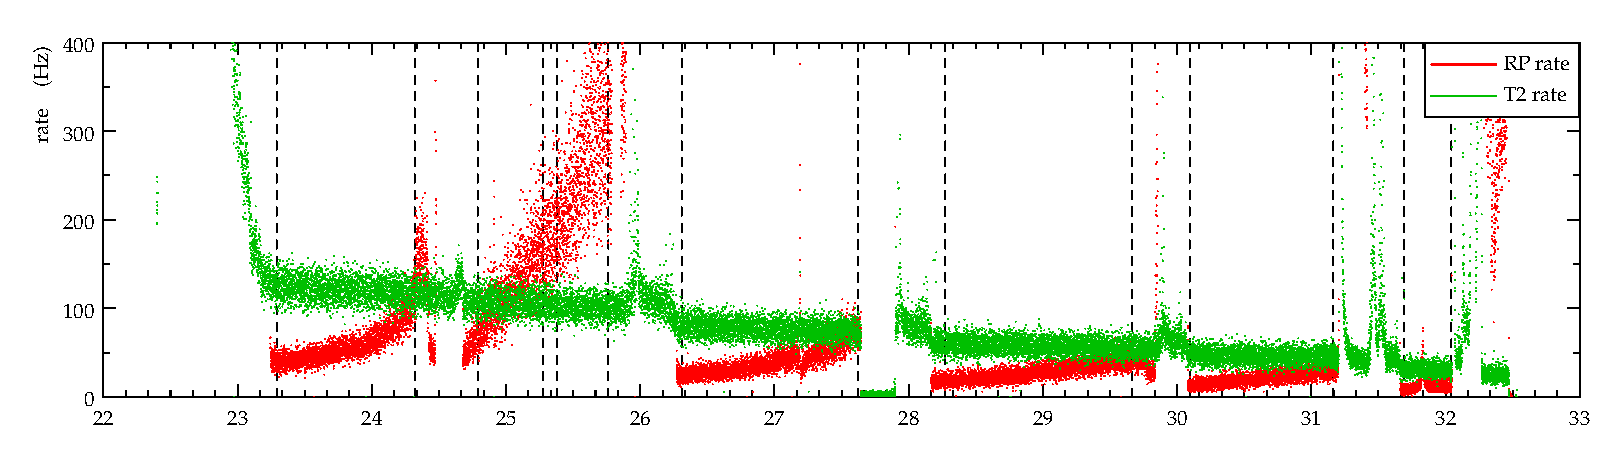
\includegraphics[width=16cm]{fig/overview.pdf}
\vskip-3mm
\caption{Illustration of the beam conditions. The T2 rate is roughly proportional to luminosity. The RP rate is sensitive to luminosity plus beam-halo. The pile-up probability follows the intensity of beam-halo protons.}
\label{fig:overview}
\end{center}
\end{figure*}


%--------------------------------------------------
\section{Differential cross-section}


%-------------------------
\subsection{Alignment}

\> the three methods: collimation, track-based and with physics processes

\> the new approach for alignment with elastics
\>> excellent for relative alignment (between near and far or left and right)
\>> absolute (= wrt.~the beam) achieved with the right arm and two complementary methods:

\noindent 1) standard method with vertical RPs
\noindent 2) fitting the axis of diffractive-proton axis and extrapolation to beam position

\> final uncertainty, also propagated to $\theta^*_{x, y}$ angles

\> the observed hit inefficiencies -- possible asymmetries -- discuss ???
\> mention final alignment check = 2D Gaussian fit of $\theta_x^*$ vs.~$\theta_y^*$ from both diagonals ??


%-------------------------
\subsection{Kinematics reconstruction}

\> choice of reconstruction formulae in x and in y
\>> guide = robustness against error sources: beam divergence, sensor pitch, misalignment, vertex term neglected, optics imperfections
\>> two types of reconstruction: one-arm (for cuts) and two-arm (for physics)
\>> TODO: what reco formulae used

\> typical values of uncertainties: statistical (smearing) and systematic (optics, ...)

%-------------------------
\subsection{Elastic tagging}

\> the three main cuts: left-right collinearity in $x$ and $y$, left-right vertex $x^*$ comparison
\>> motivation, sigmas
\> applied at 4 sigmas ??
\> inefficiency of the cuts (how many true events lost)

\> control cuts (not applied, used for validation only): $y^{N}$ vs.~local $\theta_y$ correlation, reconstructed $x^*$ compatible with vertex distribution?


%-------------------------
\subsection{Background}

\> background = impurity of the cuts above

\> method: plot a cut quantity under various cuts
\>> central peak (signal) stays
\>> tails (background) drop
\>> residual after all cuts $\rightarrow$ interpolate to signal region $\rightarrow$ background negligible
\>> can be repeated for any cut -- compatible results ??

\> further test: $|t|$-distributions under various combinations of cuts -- background distributed uniformly over $|t|$, no peaking

%-------------------------
\subsection{Efficiencies}

\> ``standard procedure'' for the standard contributions (ref. to previous publications?): ``3-out-of-4'' (uncorrelated 1-RP inefficiencies), ``shower in near'' (near-far correlated) and ``pile-up'' (coincidence with beam-halo or any other particle)

\> 3-out-of-4 results
\>> right arm: typical results (near $\approx 98\un{\%}$, far $\approx 96.5\un{\%}$ efficiency)
\>> left arm: efficiency in far RP unexpectedly low ($\approx 90\un{\%}$) -- due to showers in horizontal RPs (horizontal in left arm closer that in the right one) -- but experimentally determinable and thus fully correctable

\> pile-up results shown in Fig.~\ref{fig:overview}
\>> strong time-dependece: linear rise within the data-taking periods, decrease in beam cleanings


%-------------------------
\subsection{Acceptance correction}

\> ``standard procedure'' (ref. to previous publications?): ``divergence'' and ``phi'' corrections

\> also applied $-50 < \theta_x^* < 80\un{\mu rad}$ selection to avoid the regions affected by the horizontal RPs


%-------------------------
\subsection{Unfolding of resolution effects}

\> ``standard procedure'' (ref. to previous publications?)

\> but time-dependent smearing sigma, determined from the variation of $\theta_y^{*R} - \theta_y^{*L}$
\>> mention the subtlety with $\sigma(\theta_x^*)$ ?? Cannot be measured directly. The only handle comes from the emittances (crude only). But (at least for low-$|t|$), the impact of $\theta_x^*$ smearing is small -- the value of $\theta^*$ is mostly made by $\theta_y^*$, therefore $\theta_x^*$ must be very small. Consequently, $\Delta t_x = 2 \theta_x^* \Delta \theta_x^* \approx 0$

\> due to the very small beam divergence, the effect is negligible for all bins except the low-$|t|$ ones where the rapid cross-section growth appears because of the Coulomb interaction

%-------------------------
\subsection{Luminosity}

\> determined by fitting $\d N/\d t$ from $1000\un{m}$ to $\d\sigma/\d t$ from $90\un{m}$ (where the luminosity-independent method was applied, yielding $4\un{\%}$ uncertainty)

\> full uncertainty $\approx 5\un{\%}$


%-------------------------
\subsection{Systematic uncertainties}

\> ``standard procedure'' (ref. to previous publications?) of uncertainty assessment

\> leading uncertainties: residual misalignment (very low-$|t|$), normalisation (flat)

\> compatible results obtained if data right after or right before beam cleaning are used



%--------------------------------------------------
\subsection{Result}

\begin{figure*}
\begin{center}
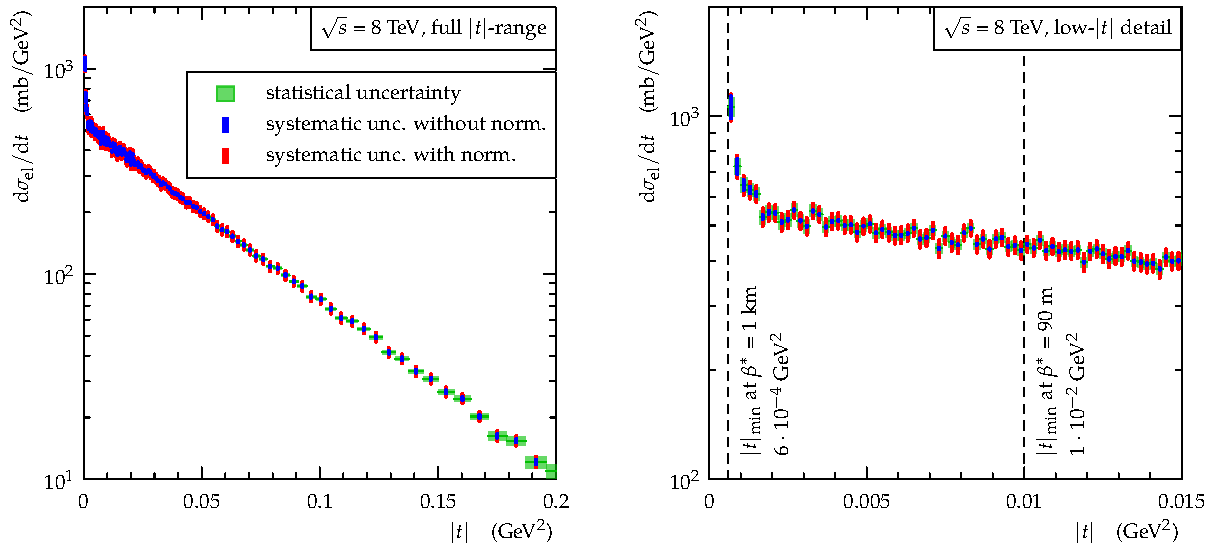
\includegraphics[width=16cm]{fig/plotTabulation.pdf}
\vskip-3mm
\caption{Differential cross-section.}
\label{fig:dsdt}
\end{center}
\end{figure*}

\> present/comment Fig.~\ref{fig:dsdt}

\> Table with points? Now or later (in a compilation with all 8 TeV data)?


%-------------------------
\section{Analysis of Coulomb-nuclear interference region}
\label{sec:cni}

\> general note: approach = not just a blind fit, but probe and test

\> key elements of phenomenology/theory of Coulomb-nuclear interference
\>> Coulomb amplitude: ``well'' known
\>> interference formula: SWY (traditionally used) or KL (theoretically more appropriate)
\>> modulus of nuclear amplitude -- strongly constrained by data $\Rightarrow$ exponential parametrisation $\d\sigma / \d t \propto \exp( -B(t) )$; reasonable degrees of the $B(t)$ polynomial are $N_b = 1, 2, 3$ (describes well the data and many phenomenological models); $N_b = 1$ gently disfavoured by the data ($B(t)$ plots, worse fits); fit amplitude anchored to $90\un{m}$ data at $|t| > 0.2\un{GeV^2}$
\>> phase of nuclear amplitude -- weak guidance from data $\Rightarrow$ need assumption: constant, central, peripheral (the last two as from \cite{kl94})

\> two goals
\>> distinction between different models/assumptions: interference formula, phase of nuclear amplitude, degree of the $B(t)$ polynomial. See section \ref{sec:cni dist mod}.

\>> determination of parameters of interest (e.g.~$\rho$, total cross-section with Coulomb taken into account), for certain reasonable models/assumptions. In section \ref{sec:cni par det}.


%-------------------------
\subsection{Parameter determination}
\label{sec:cni par det}

\> general comment: need to work with certain theoretical framework (assumption), the following chosen
\>> with SWY: only constant phase and $N_b = 1$
\>> with KL: nuclear phase constant/central/peripheral, $N_b = 1, 2, 3$ (exclude 1 ??)

\> central/peripheral phases: parametrisations as in \cite{kl94}, but refitted at $8\un{TeV}$ -- some details of the fitting ??
\>> uncertainties of the phase parameters -- {\bf waiting for the input from Vojt\v ech}.


\> generalised $\chi^2$ fits (covariance matrix contained all relevant contributions: statistical, normalisation and misalignment), fits driven by Minuit

\> extensive MC tests (input: phenomenological models as well as data fits)
\>> check for bias: only small
\>> understanding/evaluation of the method response to statistical and systematic uncertainties

\> results ($\rho$, $\sigma_{\rm tot}$, $B^{\rm N}(0)$, ...)
\>> for the model choices above -- keeping phase parameters fixed at their central values from Vojt\v ech
\>> for peripheral-phase parameters being varied within their uncertainties $\Rightarrow$ uncertainty band

\> question: do we want to present a single-value result for $\rho$ (combined from fits under different models) ??

\> discuss the new value of $\sigma_{\rm tot}$ in comparison to our previous measurement \cite{prl111}; values compatible; remind in what is the new measurement better ??

\> reference to Fig.~\ref{fig:rho_s}

\begin{figure*}
\begin{center}
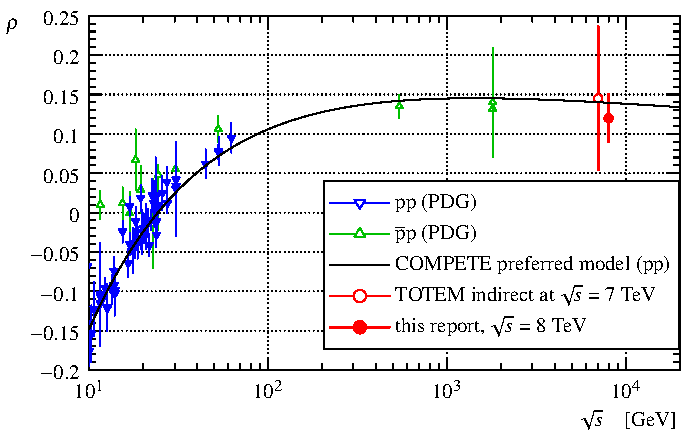
\includegraphics[width=16cm]{fig/rho_s.pdf}
\vskip-3mm
\caption{$\rho$ as a function of $s$.}
\label{fig:rho_s}
\end{center}
\end{figure*}

\> figure for $\sigma_{\rm tot}$ result ?? 

%-------------------------
\subsection{Distinction between different models}
\label{sec:cni dist mod}

\> wish to discriminate between
\>> SWY and KL interference formulae: very little difference predicted, not possible with the current data (prove/illustrate)
\>> constant/central phase: very little difference predicted, not possible with the current data (prove/illustrate)
\>> constant/peripheral phase: gentle (percent) effect at higher-$|t|$ region
\>> degree of the $B(t)$ polynomial

\> match metrics: Kolmogorov-like (explain!). Integration from right optimises sensitivity in higher-$|t|$ region where the effect of different phases is more significant (as opposed to the low-$|t|$ region mostly sensitive to $\rho$)
\>> why not using $\chi^2$: all points mixed $\Rightarrow$ not enough sensitivity

\> minimisation engines: custom developed simplex minimisation with simulated annealing (according to the Numerical Recipes)
\>> scans used to validate the algorithm

TODO: the rest


%--------------------------------------------------
\section{Discussion/Conclusions}

\> here or at the ends of sections 4 and 5 ??


%--------------------------------------------------
\section{Outlook}

\> if any...

\> what data we have and will publish in near future?


%--------------------------------------------------
\acknowledgments

\iffalse
We are indebted to the beam optics development team
%({\sc A.~Verdier} in the initial phase, {\sc H.~Burkhardt}, {\sc G.~M\" uller}, {\sc S.~Redaelli}, {\sc J.~Wenninger}, {\sc S.~M.~White})
for the design, the thorough preparations and the successful commissioning of the $\beta^* = 90\un{m}$ optics. We congratulate the CERN accelerator groups for the very smooth operation in 2011. We thank
%{\sc M.~Ferro-Luzzi}
the LHC machine coordinators for scheduling the dedicated fills.

We are grateful to CMS for providing their luminosity measurements.

This work was supported by the institutions listed on the front page and partially also by NSF (US), the Magnus
Ehrnrooth foundation (Finland), the Waldemar von Frenckell foundation (Finland), the Academy of
Finland, the OTKA grant NK 101438, 73143 (Hungary) and the NKTH-OTKA grant 74458 (Hungary).

\fi

%--------------------------------------------------
\begin{thebibliography}{99}

\bibitem{jinst}
    %The TOTEM Experiment at the CERN Large Hadron Collider, JINST 3 S08007, 2008
	\Name{Anelli G.~\etal{}~(TOTEM Collaboration)}
	\REVIEW{JINST}{3}{2008}{S08007}
\bibitem{epl95}
    %Proton-proton elastic scattering at the LHC energy of \sqrt{s} = 7 TeV, Europhys. Lett. 95 (2011) 41001,CERN-PH-EP-2011-101 
	\Name{Antchev G.~\etal{}~(TOTEM Collaboration)}
	\REVIEW{Europhys.~Lett.}{95}{2011}{41001}

\bibitem{epl96}
    %First measurements of the total proton-proton cross-section at the LHC energy of $\sqrt s =7\,\rm TeV$ CERN-PH-EP-2011-158
	\Name{Antchev G.~\etal{}~(TOTEM Collaboration)}
	\REVIEW{Europhys.~Lett.}{96}{2011}{21002}

\bibitem{epl101}
	\Name{Antchev G.~\etal{}~(TOTEM Collaboration)}
	\REVIEW{Europhys.~Lett.}{101}{2013}{21004}

\bibitem{prl111}
	\Name{Antchev G.~\etal{}~(TOTEM Collaboration)}
	\REVIEW{Phys.~Rev.~Lett.}{111}{2013}{012001}

\bibitem{kl94}
	\Name{Kundr\' at, V. and Lokaj\' i\v cek, M.}
	%title     = "High-energy scattering amplitude of unpolarized and charged hadrons",
	\REVIEW{Z.~Phys.}{C63}{1994}{619--630}
	%doi       = "10.1007/BF01557628",


\iffalse
\bibitem{P2} 
	\Name{Antchev G.~\etal{}~(TOTEM Collaboration)}
	%\REVIEW{Europhys.~Lett.}{TODO}{2012}{TODO}
	CERN-PH-EP-2012-352

\bibitem{P3} 
	\Name{Antchev G.~\etal{}~(TOTEM Collaboration)}
	%\REVIEW{Europhys.~Lett.}{TODO}{2012}{TODO}
	CERN-PH-EP-2012-353

\bibitem{jinst}
    %The TOTEM Experiment at the CERN Large Hadron Collider, JINST 3 S08007, 2008
	\Name{Anelli G.~\etal{}~(TOTEM Collaboration)}
	\REVIEW{JINST}{3}{2008}{S08007}

\bibitem{jan_thesis}
	\Name{Ka\v spar J.}
	PhD Thesis, CERN-THESIS-2011-214, {\tt http://cdsweb.cern.ch/record/1441140}

\bibitem{mario_ipac_2011}
	\Name{Deile M.}
	{\it The First 1 1/2 Years of TOTEM Roman Pot Operation at LHC}, in
	{\it Proceedings of the 2nd International Particle Accelerator Conference (IPAC 2011), San Sebastian, Spain}. 
	%{\tt http://accelconf.web.cern.ch/AccelConf/IPAC2011/papers/mopo011.pdf}
	arXiv:1110.5808v1

\bibitem{kklp}	
	\Name{Ka\v spar, J.~\etal}
	\REVIEW{Nucl.~Phys.}{B843}{2011}{84}

%\bibitem{pdg} 
%	\Name{Nakamura K.~\etal{} (Particle Data Group)}
%	\REVIEW{J.~Phys.}{G37}{2010}{075021}

\bibitem{B_vs_s}
	\Name{ISR (CR Collaboration)} \REVIEW{Phys.~Lett.}{B62}{1976}{460}; 
	\Name{ISR (ACHGT Collaboration)} \REVIEW{Phys.~Lett.}{B39}{1972}{663}; 
	\Name{ISR (R-211)} \REVIEW{Nucl.~Phys.}{B262}{1985}{689}; 
	\Name{ISR (R-210)} \REVIEW{Phys.~Lett.}{B115}{1982}{495}; 
	\Name{UA1} \REVIEW{Phys.~Lett.}{B147}{1984}{385}; 
	\Name{UA4} \REVIEW{Phys.~Lett.}{B127}{1983}{472} and \REVIEW{Phys. Lett.}{B198}{1987}{583}; 
	\Name{UA4/2} \REVIEW{Phys.~Lett.}{B316}{1993}{448}; 
	\Name{CDF} \REVIEW{Phys.~Rev.}{D50}{1994}{5518}; 
	\Name{E710} \REVIEW{Phys.~Rev.~Lett.}{68}{1992}{2433} and \REVIEW{Nuovo Cimento}{A106}{1992}{123}; 
	\Name{D0} D0 Note 6056-CONF; 
	\Name{pp2pp} \REVIEW{Phys.~Lett.}{B579}{2004}{245}

\bibitem{lafferty94}
 	% Where to stick your data points: The treatment of measurements within wide bins
	\Name{Lafferty G.~D.~and Wyatt T.~R.}
	\REVIEW{Nucl.\ Instrum.\ Meth.}{A 355}{1995}{541}

\bibitem{compete} 
	\Name{Cudell~J.~R.~\etal{} (COMPETE Collaboration)}
	\REVIEW{Phys.\ Rev.\ Lett.}{89}{2002}{201801}

\fi

\end{thebibliography}

\end{document}
